%
%   
%   IA Project ATARI-GO
%   UNIVERSITY OF NANTES
%   MASTER ALMA 1
%   2009 - 2010
%   Version 1.0
%   
%   $Date$
%   $Author$
%   $Revision$
% 
%   Copyright (C) 2010 Romain Gournay & Bruno Belin, All rights reserved.
% 
%   This program is free software: you can redistribute it and/or modify
%   it under the terms of the GNU General Public License as published by
%   the Free Software Foundation, either version 3 of the License, or
%   (at your option) any later version.
%
%   This program is distributed in the hope that it will be useful,
%   but WITHOUT ANY WARRANTY; without even the implied warranty of
%   MERCHANTABILITY or FITNESS FOR A PARTICULAR PURPOSE.  See the
%   GNU General Public License for more details.
%
%   You should have received a copy of the GNU General Public License
%   along with this program.  If not, see <http://www.gnu.org/licenses/>.
%
%	
\documentclass[a4paper,12pt]{report}
\usepackage[utf8x]{inputenc}
\usepackage{graphicx}
\usepackage{verbatim}
% Title Page
\title{Atari-Go Project  \\  \bigskip{} Technical File}
\author{
Belin Bruno \&
Gournay Romain
}


\begin{document}
\maketitle



\begin{abstract}
      
This document is the technical file of the artificial intelligence project. It describes the designing of the application and the algorithms used.

\end{abstract}

\tableofcontents

\chapter{Introduction}
\label{chap:Designing}

\section{Context}
\paragraph*{}
This document correponding to the technical file from Atari-go Game developped by Bruno Belin \& Romain Gournay. 
\paragraph*{}
This work is done during the second half of 2010 in the course of Artificial Intelligence of the Master in Computer Science ALMA 1st year of the University of Nantes.

\section{Objective}
\paragraph*{}
The goal is to complete the implementation of a program that allows a human to play the atari-go game against the computer. This work aims to implement algorithms, concepts and methods seen in the course of IA. The program will seek to play the best possible using algorithmic strategies such as min-max and alpha-beta. We define an evaluation function as relevant as possible.


\chapter{Design}
    \paragraph*{}
    In this section, we present the organization and content of the different packages of the application. 
    Given the number of classes, we will explain briefly the details of each component.
    The program is cut in three main parts, packages :

    \begin{center}
	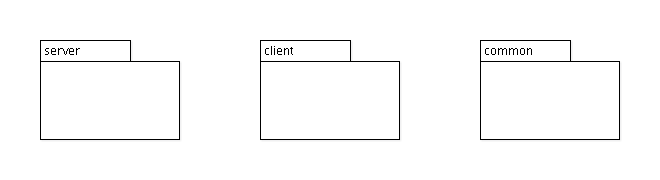
\includegraphics[width=0.75\textwidth]{img_rapport/designing_1.png}
    \end{center}

    \begin{itemize}
	\item The \textit{server} package contains all classes which used to play in the program.
	\item The \textit{client} package contains all the HMI components
	\item The \textit{common} package contains all the the common elements between the server and the client packages.
    \end{itemize}
 
    Firstable, we present the general architecture of the application in section below.
    \section{Architecture of the application}
    \begin{center}
	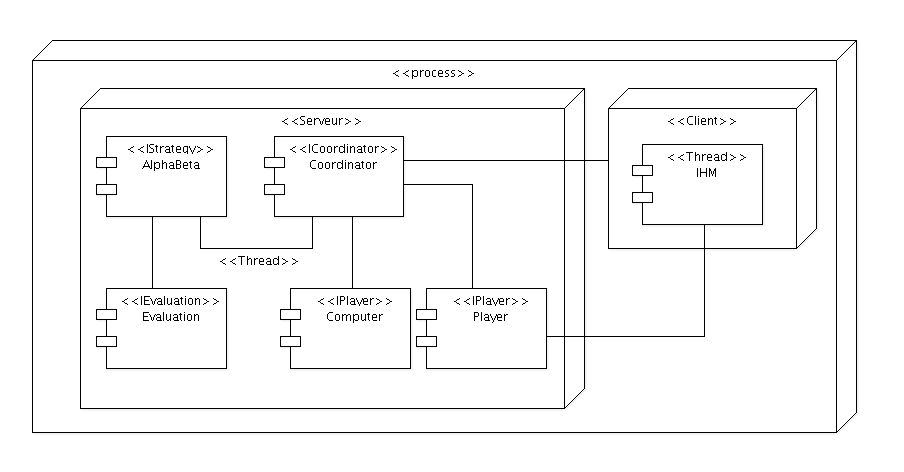
\includegraphics[width=0.75\textwidth]{img_rapport/designing_0.png}
    \end{center}
    \paragraph*{}
    The ``\textit{Client}`` part is the Swing GUI components. It is isolated from the rest of the application. We'll find it in the client package.
    
    \paragraph*{}
      The ''\textit{server}'' part is the program that plays. It communicates with the HMI in two points:
      \begin{itemize}
	\item through the coordinator to request the Goban refresh after each turn and to indicate the end of the game through a single dialog box.
	\item via the player (player who confronts the computer) to detect mouse actions.
    \end{itemize}

    \paragraph*{}
      Communication with the HMI is based on the Observer design pattern. In this way, we maintain a strong decoupling between different layers,
      the communication being by exchanging messages. Swing already provides this type of communication through Listeners (addMouseListener, ...).
    \paragraph*{}
    The Coordinator has a key function as a conductor: it coordinates the actions between the player and computer.
    It invoke AlphaBeta to determine the best move when the computer is playing. It allows the player to play when it is his turn.
    To do this, we make available to a listener (PlayerListener) to observe the actions of one or the other way and completely independent of Swing.
    
    \paragraph*{}
    Even if it only manages a single strategy or evaluation function in our implementation,
    the application will be able to easily integrate other components thanks to a layer of abstraction (IStrategie, IEvaluation) and using a Factory.
    

    \section{Package fr.alma.server}
	The package server is itself composed of three sub packages.
	\begin{center}
	    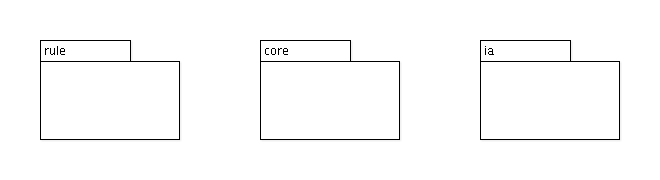
\includegraphics[width=0.75\textwidth]{img_rapport/designing_2.png}
	\end{center}
	\begin{itemize}
	    \item The \textit{rule} package contains all classes linked to the game rules.
	    \item The \textit{core} package groups the main classes such as Coordinator or the differents Interfaces.
	    \item The \textit{ia} package corresponds mainly to the brain of the computer game play.
	\end{itemize}

      \subsection{Package fr.alma.server.rule}
	  The rule package contains all classes relating to the management rules of the game:
	  \begin{center}
	      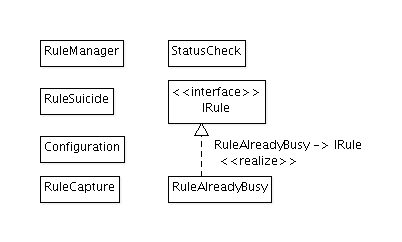
\includegraphics[width=0.75\textwidth]{img_rapport/designing_3.png}
	  \end{center}

	  \begin{itemize}
	      \item The \textit{Configuration} class specify the color that should begin to play (static rule).
	      \item \textit{RuleManager} integrates the different rules applicable to a dynamic context.
	      \item \textit{StatusCheck} is the result of a dynamic control for a location returned by the class \textit{RuleManager}.
	  \end{itemize}


      \subsection{Package fr.alma.server.core}
	  \paragraph*{}
	  This package contains the generic components that support the internal operation of the game.
	  \paragraph*{}
	  The classes \textit{Computer} and \textit{Player} reprensent both players of the applications. They reused AbstractPlayer code for common parts.
	  \paragraph*{}
	  Player sets up a listener on the Goban Swing through addMouseListener method. This allows it to respond to user mouse clicks. 
	  He transcribes and transmits the significant events in the class Coordinator.
	  \paragraph*{}
	  For \textit{Computer} things are a little different. When the class \textit{Coordinator} ask its to play, it updates the status bar (GUI) to indicate that it plays and seeks Strategy program it is associated with a suddenly find the least negative possible. 
	  Once he gets the result he immediately forward the information to \textit{Coordinator}.
	  \paragraph*{}
	  As discussed above, Class \textit{Coordinator} acts as a conductor. It listens to the events of both players and react accordingly. 
	  It is its which asks the Panel to find out what is the color that should begin to play. Then, it asks to the player corresponding to the color. 
	  When it shalls transmit the desired location, it carries the appropriate controls and either accept or reject the move. 
	  If it is a winning move, it shows who won and ended the game. Otherwise, it passes control to another player.
	  \paragraph*{}
	  \textit{StateGame} represents a state of the game at this level we find all the places occupied by players and those still available.
	  \paragraph*{}
	  \textit{Location} allows you to specify a location on the Goban (column, row).
	  \paragraph*{}
	  \textit{PlayerListener} and \textit{PlayEvent} allow the communication of messages between the players and the \textit{Coordinator}.
	  The \textit{Coordinator} position at the beginning of game a \textit{PlayerListener} on each player to keep informed of its actions and at the same time controlling them.
	  Indeed, every event from a player is intercepted by the \textit{Coordinator} which may cancel its spread and therefore the associated actions.
	  For example, if the user (player) click on an intersection of the Goban already occupied or that do not comply with a rule, the Coordinator will respond is denied actions.
	  \paragraph*{}
	  The Component \textit{Factory} allows to instantiate all components to retrieve specific the appropriate interfaces.
	  This allows to maintain independence from concrete implementations to facilitate future changes of the application.

	  \begin{center}
		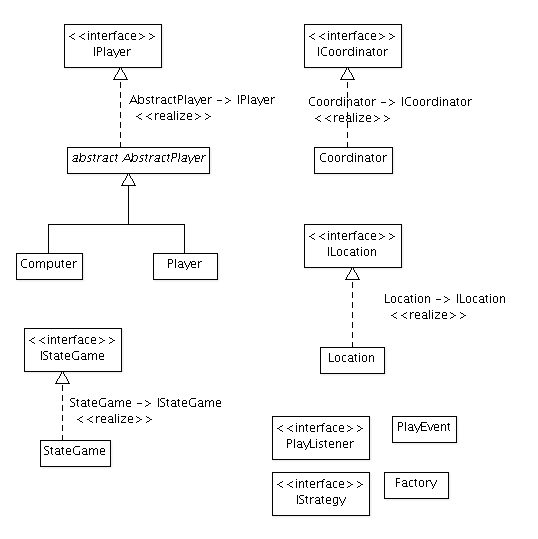
\includegraphics[width=0.75\textwidth]{img_rapport/designing_4.png}
	  \end{center}

      \subsection{Package fr.alma.server.ia}
	  \paragraph*{}
	      We touch here on the "brain" of the application : all classes in direct link with artificial intelligence.
	      \begin{center}
		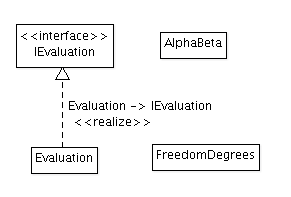
\includegraphics[width=0.75\textwidth]{img_rapport/designing_5.png}
	      \end{center}
	  \paragraph*{}
		\textit{Evaluation} is the evaluation function and the \textit{AlphaBeta} algorihm to the same name algorithm.

	  \paragraph*{}
	      We note that \textit{AlphaBeta} is an implementation of the \textit{IStrategy} interface from the core package (mentioned above).

	  \paragraph*{}
	      The application has been designed to easily change these elements statically or dynamically (during the game).

    \section{Package fr.alma.client}
	\paragraph*{}
	    This section is to isolate all elements related to the GUI. We thus find all classes that implement the Swing API.
	     \begin{center}
	      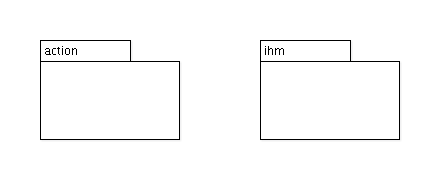
\includegraphics[width=0.75\textwidth]{img_rapport/designing_6.png}
	    \end{center}
	  
	\subsection{Package fr.alma.client.action}
	    \paragraph*{}
		\begin{center}
		    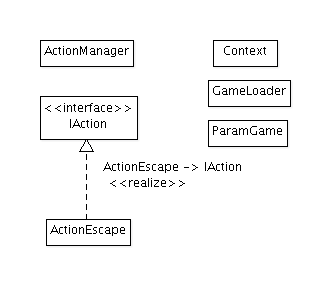
\includegraphics[width=0.75\textwidth]{img_rapport/designing_7.png}
		\end{center}

		\textit{ActionManager} defined all the actions available from the application menu.
	    
	    \paragraph*{}
		\textit{ActionEscape} is the treatment to be used when the user uses the Escape key to interrupt the computer calculations.
	       
	    \paragraph*{}
		\textit{GameLoader} is used to load a saved game as a text file. It is implemented in our unit tests to verify the no-regression of our application.
		We can thus verify the operation of AlphaBeta, detection catches and check the results of our evaluation function.

	    \paragraph*{}
		\textit{ParamGame} contains the parameters of a game. When the player requests a new game, he defines the configuration of the game through the GUI's menu.
		The different criteria are then recovered from the graphics components to power the \textit{ParamGame} component which has no connection with Swing.
		Then, this component can be spread in the game engine without causing friction respecting to the graphics layer.
	   
	    \paragraph*{}
		\textit{Context} is the context of the game It encapsulates different components to share them. Thus, it transmits the Context toward the different classes, thus avoiding to transmit all the elements one by one.
,
	\subsection{Package fr.alma.client.ihm}
	  \paragraph*{}
	      These classes are the graphic representation of our application of atari-go.
	      \begin{center}
		    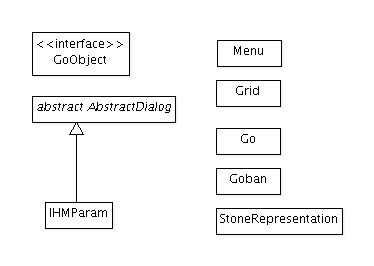
\includegraphics[width=0.75\textwidth]{img_rapport/designing_8.png}
		\end{center}

	  \paragraph*{}
	      \textit{IHMParam} allows to entry parameters of a new game.

	  \paragraph*{}
	      \textit{Menu} supports the application menu. It is a simple menubar.
	   
	  \paragraph*{}
	      \textit{Goban} integrates and supports the representation of the grid (\textit{Grid}) and stones (\textit{StoneRepresentation}).
	      It is at this level that we use the status of the game to know what stones to display.
	  \paragraph*{}
	      The class \textit{Go} is the entry point of the application. This class supports the construction of the main window, the establishment of the menu
	      (which will launch a new party) and the listener to intercept the strike on the Escape key.

\chapter{Algorithms}
     \paragraph*{}
     In this section, we present the important algorithms are artificial intelligence computer. Among these algorithms there are:
      \begin{itemize}
	  \item Min-Max, AlphaBeta algorithms
	  \item Evaluation Function
      \end{itemize}

      \section{Min-Max, AlphaBeta algorithms}
	  \paragraph*{}
	  As part of this project, it is asked to use Min-Max and Alpha-Beta in connection with an evaluation function as relevant as possible.
	  \paragraph*{}
	  Insofar as Alpha-Beta is an extension of Min-Max much more efficient and giving the same results on the strategy,
	  we focus on the AlphaBeta technique.
	  \paragraph*{}
	  This algorithm works on a tree where each level is either the player's opportunities to play or computer opportunities to play, starting from the root
	  which correponds to the current situation, to down to the leaves that are either end of a party or a maximum depth of research.
	  This depth should reflect the size of the Goban. It has been adjusted to obtain good response times compared to the results of our tests.
	  \paragraph*{}
	  To introduce new elements and to be closer to reality, we propose to introduce this algorithm in two structures:
.	  \paragraph*{Value}
	  Corresponds to the minimum or maximum value found for the given location.
	  {Value, location}
	  \paragraph*{StatusCheck}
	  Corresponds to the elements of the last inspection done compared to the rules engine (see the method calls checkBefore).
	  {PossibilityToPlay, gameOver, winner, location}
	  \begin{center}
	  \begin{verbatim}
Function getBestLocation(functionEvaluation, stateGame)
Begin 
  evaluation = functionEvaluation;
  stateGameCloned = clone(stateGame); 
  interruption = false; 
  Value value =  getValue(2, stateGameCloned,+oo, null); 
  return  value.location;
End 
	  \end{verbatim} 


	  \begin{verbatim}
Fonction getValue(level, stateGame, extremum, checkStatus)
Begin 
  If(level < LevelMax) 
      && existChild(checkStatus) 
      && (!interruption) Then
    If (level is pair) Then
      value = max(level, stateGame, extremum);
    Else
      value = min(level, stateGame, extremum);
    End If
  Else
    stateGame.level = level;
    value = 
      new Value(evaluation(stateGame, checkStatus), null);
  End If
  return value;
End
	  \end{verbatim} 

	  \begin{verbatim}
Function max(level, stateGame, extremum)
Begin
  Value max = new Value(-oo);
  For each free location in the stateGame Do
    If (max.value < extremum) Then
      checkStatus =
	  checkBefore(stateGame, location, computer) ;
      If (checkStatus.PossibilityToPlay) Then
	play on this location for the computer on stateGame;
	Value value = 
	    getValue(level+1, stateGame, max.value,  checkstatus);
	If (value.value > max.value) Then
	  max = value;
	  max.location = location;
	End If
	free the location on stateGame;
      End If
    End If
  End For
  return max;
End
 \end{verbatim}

	  \begin{verbatim}
Function min(level, etatDuJeu, extremum)
Debut
  Valeur min = new Value(+oo);
  For each free location in the stateGame Do
    If (max.value > extremum) Then
      checkStatus = checkBefore(stateGame, location, player)
      If (checkStatus.PossibilityToPlay) Then
	play on this location for the player on stateGame ;
	Value value = 
	  getValue(level+1, stateGame, min.value,  checkstatus);
	If (value.value > min.value) Then
	  min = value;
	  min.location = location;
	End If
	free the location on stateGame;
      End If
    End If
  End For
  return min;
End
 \end{verbatim}
	\end{center}
      \section{Evaluation Function}
	  \paragraph*{}
	  The evaluation function is, as its name suggests, to evaluate a game situation without considering the context.
	  It identify the relevance of each move and guide strategic choices.
	  \paragraph*{}
	  these are the rules of atari-go, the player who makes the first catching, wins.
	  The number of captured stones is irrelevant. We will evaluate a game state based play opportunities on the computer and the player.
	  \paragraph*{}
	  The possibilities of play are determined by reference to degrees of freedom of different stones or groups of connected stones.
	  The software must answer to the following questions for each color of stone:
	  \begin{itemize}
	   \item How many are there stones or groups of stones associated with a degree of freedom to zero
	   \item How many are there stones or groups of stones associated with a degree of freedom to one
	   \item etc.
	  \end{itemize}
	  \paragraph*{}
	  The function apply then a decreasing weight to each response, starting with a maximum weight for the freedoms to zero.
	  \paragraph*{}
	   The score of the computer corresponds to the playable opportunities of the opposing color.
	  \paragraph*{}
	  The result returned by the evaluation function is the difference between the score obtained by the computer and that obtained by the player:
	  a positive value to a situation positive for the computer, and negative in the opposite case.
	  
	  \paragraph*{}
	  This algorithm uses two functions that are intermediate and cumulFreedomDegrees and getScore.
	  \paragraph*{cumulFreedomDegrees}
	   calculates the number of blocks or groups with n freedom degrees 
	  and store in a table used to calculate the score of a state of the game
	  \paragraph*{getScore}
	    allows, as its name suggests to return a score for a state game based on the table calculated by the function cumulFreedomDegrees.
	   \paragraph*{}
	      \begin{verbatim}
Function Evaluation(stateGame,  checkStatus)
Begin
  If (checkStatus.isGameOver) Then
    If (checkStatus.vainqueur == computer ) Then
      score = 1000000 /  (stateGame.level – 2);
      return  score;
    Else
      score = -1000000 /  (stateGame.level – 2);
      return  score;
    End If
  End If

  ScoreOrdinateur =
	getScore(cumulFreedomDegrees(computer, stateGame));
  ScoreJoueur =
	getScore(cumulFreedomDegrees(player, stateGame));
  return   ScroreComputer -  ScorePlayer;
End
 \end{verbatim}

      \begin{verbatim}
Function cumulFreedomDegrees(aPlayer,  stateGame)
Begin
  AlreadyVisitedLocations = null;
  arrayFreeDegrees = null;
  For each location of the Goban Do
    If ((aPlayer == computer) && (location == joueur)) or 
	((aPlayer == player) && (location == computer)) Then
      If emplacement is not in AlreadyVisitedLocations Then
	freeDegrees =
	  CountFreeDegrees(location, AlreadyVisitedLocations);
	incrément the conten in arrayFreeDegrees[freeDegrees];
      End If
    End If
  End For
  return arrayFreeDegrees ;
End
 \end{verbatim}

  \begin{verbatim}
Function getScore(arrayFreeDegrees)
Begin
  cumul = 0;
  For each element of arrayFreeDegrees Do
      (if indice > 4 then x= 0 else x= 5-indice);
      weigth = 10 to the power x
      cumul = cumul + (arrayFreeDegrees(indice) * weigth);
  End For
  return cumul;
End

 \end{verbatim}


\end{document}    